\documentclass[10pt,landscape]{article}
\usepackage{multicol}
\usepackage{calc}
\usepackage{ifthen}
\usepackage[landscape]{geometry}
\usepackage{listings}
\usepackage{amsmath,amsthm,amsfonts,amssymb}
\usepackage{mathtools}
\usepackage{color,graphicx,overpic}
\usepackage{hyperref}
\usepackage[dvipsnames]{xcolor}

\usepackage{MnSymbol}
\usepackage{graphicx}
\usepackage{wrapfig}

% This sets page margins to .1 inch if using letter paper, and to 1cm
% if using A4 paper. (This probably isn't strictly necessary.)
% If using another size paper, use default 1cm margins.
\ifthenelse{\lengthtest { \paperwidth = 11in}}
    { \geometry{top=.1in,left=.1in,right=.1in,bottom=.1in} }
    {\ifthenelse{ \lengthtest{ \paperwidth = 297mm}}
        {\geometry{top=1cm,left=1cm,right=1cm,bottom=1cm} }
        {\geometry{top=1cm,left=1cm,right=1cm,bottom=1cm} }
    }

% Turn off header and footer
\pagestyle{empty}

% Redefine section commands to use less space
\makeatletter
\renewcommand{\section}{\@startsection{section}{1}{0mm}%
                                {-1ex plus -.5ex minus -.2ex}%
                                {0.5ex plus .2ex}%x
                                {\normalfont\large\bfseries}}
\renewcommand{\subsection}{\@startsection{subsection}{2}{0mm}%
                                {-1ex plus -.5ex minus -.2ex}%
                                {0.5ex plus .2ex}%
                                {\normalfont\normalsize\bfseries}}
\renewcommand{\subsubsection}{\@startsection{subsubsection}{3}{0mm}%
                                {-1ex plus -.5ex minus -.2ex}%
                                {0.5ex plus .2ex}%
                                {\normalfont\small\bfseries}}
\makeatother

% Itemize to use less space
\usepackage{enumitem}
\setlist{leftmargin=*, nosep}
\setenumerate{nosep}

% Define BibTeX command
\def\BibTeX{{\rm B\kern-.05em{\sc i\kern-.025em b}\kern-.08em
    T\kern-.1667em\lower.7ex\hbox{E}\kern-.125emX}}

% Don't print section numbers
\setcounter{secnumdepth}{0}


\setlength{\parindent}{0pt}
\setlength{\parskip}{0pt plus 0.5ex}

%My Environments
\newtheorem{example}[section]{Example}

\newcommand{\Blue}[1]{\noindent{\textbf{\textcolor{Blue}{#1 -}}}}
\newcommand{\Red}[1]{\noindent{\textbf{\textcolor{BrickRed}{#1 -}}}}
\newcommand{\Green}[1]{\noindent{\textbf{\textcolor{PineGreen}{#1 -}}}}
\newcommand{\Hint}[1]{\noindent{\textcolor{Orange}{#1}}}
% -----------------------------------------------------------------------

\begin{document}
\raggedright
\footnotesize
\begin{multicols}{4}


% multicol parameters
% These lengths are set only within the two main columns
%\setlength{\columnseprule}{0.25pt}
\setlength{\premulticols}{1pt}
\setlength{\postmulticols}{1pt}
\setlength{\multicolsep}{1pt}
\setlength{\columnsep}{2pt}

\Green{Handy Transformations}
\begin{displaymath}
    \boxed{
        \begin{aligned}
            \mathbb{E}\left[a + b X\right] &= a + b\mathbb{E}\left[X\right] \\
            \mathbb{E}\left[X^2\right] &= \text{Var}(X) + \left(\mathbb{E}\left[X\right]\right)^2 \\
            \text{\textit{(ditto but flipped) }} \text{Var}(X) &= \mathbb{E}\left[X^2\right] - \left(\mathbb{E}\left[X\right]\right)^2 \\
            \text{Var}(a + b X) &= b^2 \text{Var}(X) \\
            \text{SD}(a + b X) &= |b| \text{SD}(X) \\
            \text{Cov}\left(a + b X, c + d Y\right) &= b \cdot d \cdot \text{Cov}(X, Y) \\
            \text{Corr}\left(a + b X, c + d Y\right) &= \text{Corr}(X, Y) \\
        \end{aligned}
    }
\end{displaymath}

\Green{Uniform distribution facts from HW}
\begin{enumerate}
    \item If $U \sim \text{Unif}[0,1]$, then for any fixed $a > 0$ and $b \in \mathbb{R}$, we have that $aU+b \sim \text{Unif}[b,a+b]$.
    \item If $U \sim \text{Unif}[0,1]$, then $\mathbb{E}[U] = \frac{1}{2}$ and $\text{Var}(U) = \frac{1}{12}$.
\end{enumerate}

\section{When I am not protected from me being me}

Set Algebra:
\begin{itemize}
    \item \Blue{Union} $A$ or $B$; $A \cup B$.
    \item \Blue{Intersection} $A$ and $B$; $A \cap B$.
    \item \Blue{Complement} not $A$; $A^C$.
    \item \Blue{Difference} $A$ but not $B$; $A \backslash B$
    \item \Blue{Disjoint Events aka. mutually exclusive} events $A$ and $B$ are disjoint if they don't share any
        outcomes in common (i.e., $A \text{ and } B = \emptyset$).
    \item \Blue{Subset} $A \subseteq B$
\end{itemize}

\Blue{Trial} a repetition of a random experiment/process. Trials're \underline{independent}: none gives information about the
others; are \underline{stable}: reuslts could have appeared in any order.

\Blue{Outcome} a possible result of a trial.

\Blue{Sample space} the set of all possible outcomes. Often denoted as $S$.

\Blue{Event} a set of outcomes of an experiment (i.e., a subset of the sample space).

\Red{Probability} is a long run proportion of an outcome in repeated trials.
\begin{itemize}
    \item Probabilities act as ``targets" of estimation
    \item Proportions based on data ``estimate'' probabilities. Would approach probabilities if observe infinite trials.
\end{itemize}
Formally, \fbox{$A \mapsto \mathbb{P}(A), \mathbb{P}(A) \in \left[0, 1\right]$}
A probability $\mathbb{P}(\cdot)$ on a sample space $S$ is a function that assigns a snumber between 0 and 1 to all
events, $A$ in the sample space (i.e., any possible subset of the sample space) and subject to three requirements
(axioms):
\begin{enumerate}
    \item $\mathbb{P}(S) = 1$: probability of \textit{something} in the sample space happening is 1
    \item $\mathbb{P}(A) \ge 0, \forall A$
    \item $A \text{ and } B = \emptyset \text{ (A, B disjoint) } \Rightarrow \mathbb{P}(A \cup B) = \mathbb{P}(A) + \mathbb{P}(B)$
\end{enumerate}

More takeaways
\begin{itemize}
    \item $A \subseteq B \Rightarrow \mathbb{P}(A) \le \mathbb{P}(B)$
    \item $A$, $B$, $C$ are pairwise disjoint $\Rightarrow \mathbb{P}(A \cup B \cup C) = \mathbb{P}(A) + \mathbb{P}(B) + \mathbb{P}(C)$
    \item $\mathbb{P}(A \cup B) = \mathbb{P}(A) + \mathbb{P}(B) - \mathbb{P}(A \text{ and } B)$
\end{itemize}

\Red{Joint Probability} $\mathbb{P}(A \text{ and } B)$ is the joint probability that events $A$ and $B$ occur.

\Red{Conditional Probability} $\mathbb{P}(A | B) = \frac{\mathbb{P}(A \text{ and } B)}{\mathbb{P}(B)}, \mathbb{P}(B) > 0$ the
probability of observing event $A$ if (given that) one has observed $B$. Bear in mind: $\mathbb{P}(A | B) \neq \mathbb{P}(B | A)$

\Green{Product Rule} $\mathbb{P}(A \text{ and } B) = \mathbb{P}(B) \cdot \mathbb{P}(A | B)$.

\Red{Independent Events} $A$ and $B$ are independent if $\mathbb{P}(A \text{ and } B) = \mathbb{P}(A) \cdot \mathbb{P}(B)$; one
event happening doesn't affect the probability of the other event happening. Can easily deduce that
$\mathbb{P}(A | B) = \mathbb{P}(A)$ and $\mathbb{P}(B | A) = \mathbb{P}(B)$.

\Hint{Independence and Disjointness are \textbf{NOT} synonyms.}
\begin{itemize}
    \item Independent $\Rightarrow \mathbb{P}(A \text{ and } B) = \mathbb{P}(A) \cdot \mathbb{P}(B)$
    \item Disjoint $\Rightarrow \mathbb{P}(A \text{ and } B) = 0$. Disjoint events are extremely dependent: If one event
        occurs, the other cannot.
\end{itemize}

\Red{Random variable} a numerical function on a sample space with probabilities. (Think as a scoring mechanism.)
\begin{itemize}
    \item Input: an outcome in the sample space
    \item Output: a number
\end{itemize}

\Blue{Discrete RVs} only countably many values are possible

\Blue{Continous RVs} can take on uncountably infinitely many values

\Red{Probability Distribution Function (PDF)} \fbox{$\mathbf{p}_X(x) = \mathbb{P}(X = x)$} is the probability that the
random variable $X$ takes on the value $x$. I really hate $\mathbf{p}_X(x)$ this styling, so only $\mathbb{P}(X = x)$
moving forward.

\Blue{Properties of PDFs} any function that satisfies the following conditions is a probability distribution function of
a \underline{Discrete} random variable:
\begin{enumerate}
    \item $\mathbb{P}(X = x) \ge 0, \forall x \in \mathbb{R}$ (for any real number)
    \item $\mathbb{P}(X = x) > 0$ for values that the random variable $X$ can actually take on
    \item $\mathbb{P}(X = x) = 0$ for values that aren't possible for the random variable $X$
    \item $\sum_x \mathbb{P}(X = x) = 1$
\end{enumerate}

\Red{Expected Value} \fbox{$\mathbb{E}\left[X\right] = \sum_x x \cdot \mathbb{P}(X = x)$}

\Red{Variance} a probability weighted mean of the possible squared deviations.
\begin{displaymath}
    \boxed{
        \begin{aligned}
            \text{Var}(X) &= \mathbb{E}\left[(X - \mathbb{E}[X])^2\right]\\
            &= \sum_x (x - \mathbb{E}[X])^2 \cdot \mathbb{P}(X = x) \\
            &= \mathbb{E}\left[X^2\right] - \left(\mathbb{E}\left[X\right]\right)^2
        \end{aligned}
    }
\end{displaymath}

\Red{Standard Deviation} \fbox{$\text{SD}(X) = \sqrt{\text{Var}(X)}$}

\Green{Given $Y = g(X)$ and $X$'s PDF}
\begin{displaymath}
    \boxed{
        \begin{aligned}
            \mathbb{E}\left[Y\right] &= \sum_x g(x) \cdot \mathbb{P}(X = x) \\
            \text{Var}(Y) &= \sum_x \left(g(x) - \mathbb{E}\left[g(X)\right]\right)^2 \cdot \mathbb{P}(X = x) \\
        \end{aligned}
    }
\end{displaymath}

\Red{RVs with only 2 outcomes} (not necessarily Bernoullis yet)
Suppose RV $X$'s PDF is: $\begin{cases}
    \mathbb{P}(X = a) &= p \\
    \mathbb{P}(X = b) &= 1- p \\
    \mathbb{P}(X = \text{all other values}) &= 0 \\
\end{cases}$, then:
\begin{displaymath}
    \boxed{
        \begin{aligned}
            \mathbb{E}\left[X\right] &= ap + b(1-p) \\
            \text{Var}(X) &= (a-b)^2p(1-p) \\
            \text{SD}(X) &= |a-b| \sqrt{p (1-p)}
        \end{aligned}
    }
\end{displaymath}

\Red{Bernoulli Random Variable} aforementioned when $\begin{cases}
    a &= 1 \\
    b &= 0
\end{cases}$.
If \fbox{$X \sim \text{Bern}(p)$}, then:
\begin{displaymath}
    \boxed{
        \begin{aligned}
            \mathbb{E}\left[X\right] &= p \\
            \text{Var}(X) &= p(1-p) \\
            \text{SD}(X) &= \sqrt{p (1-p)}
        \end{aligned}
    }
\end{displaymath}
\Hint{
    \begin{itemize}
        \item Variance maximized when $p = 0.5$
        \item Variance minimized when $p = 0$ or $1$
    \end{itemize}
}
Useful for tracking \underline{how many} successes happen in $n$ independent trials.

\Red{Binomial Random Variable}
If \fbox{$X \sim \text{Binom}(n, p)$}, then:
\begin{displaymath}
    \boxed{
        \begin{aligned}
            \mathbb{E}\left[X\right] &= n \cdot p \\
            \text{Var}(X) &= n \cdot p(1-p) \\
            \text{SD}(X) &= \sqrt{n \cdot p(1-p)}
        \end{aligned}
    }
\end{displaymath}

\Red{Binomial Problems} following must hold:
\begin{enumerate}
    \item Constant success probability $p$ and failure probability $(1-p)$.
    \item Fixed total number of trials: $n$
    \item trials are \underline{\textbf{independent}}
    \item Only two outcomes of interest (success or failure) on each trial
    \item \Hint{Want to find the probability of observing $k$ successes among the total number of $n$ trials}. (Order doesn't matter.)
\end{enumerate}
\fbox{$\mathbb{P}(k \text{ successes in } n \text{ trials}) = \binom{n}{k} p^k (1-p)^{n-k}$}

\Blue{Combination} how many ways to choose $k$ out of $n$: \fbox{$\binom{n}{k} = \frac{n!}{k!(n-k!)}$}.

\Red{Binomial Distribution} \fbox{$X \sim \text{Binom}(n, p)$} where $X$ is an RV tracking the number of successes in
$n$ independent trials with success probability $p$. $X$'s PDF:
\fbox{$\forall k \in \left\{0, \dots, n\right\}, \mathbb{P}(X = k) = \binom{n}{k} p^k (1-p)^{n-k}$}.
\Hint{Attn: $X$ here is not for one single trial!}.
\begin{itemize}
    \item A \textbf{Bernoulli RV}: useful for one trial's success/failure.
    \item A \textbf{Binomial RV}: useful for total number of successes.
\end{itemize}
\Blue{Binomial as the Sum of Bernoullis} $n$ independent Bernoulli RVs each with the same success probability $p$:
$\forall i \in {1, \dots, n}, X_i \sim \text{Bern}(p)$.
Define \fbox{$S_n = \sum_{i=1}^{n} X_i$}, then denote \fbox{$S_n \sim \text{Binom}(n, p)$}.
\Hint{$\text{Binom}(1, p) = \text{Bern}(p)$}

\Red{Joint Distribution of 2 RVs} the probability that 2 RVs simultaneously take on 2 values.
$\forall x \in X, \forall y \in Y$ \fbox{$\mathbb{P}(X = x, Y = y)$}.

\Green{Marginal probability distribution} can be found given with the joint PDF:
\fbox{$\mathbb{P}(X = x) = \sum_{y} \mathbb{P}(X = x, Y = y)$}

\Red{Z-Score of a Random Variable $X$}
\fbox{$Z(X) = \frac{X - \mathbb{E}\left[X\right]}{SD(X)}$}

\Hint{$\mathbb{E}\left[Z(X)\right] = 0$ and $SD(Z(X)) = 1$}

\section{Correlation and Covariance}

\Red{Correlation Between RVs $X$ and $Y$} ``average of the product of z-scores''
\begin{displaymath}
    \boxed{
        \begin{aligned}
            \text{Corr}(X, Y) &= \mathbb{E}\left[Z(X) \cdot Z(Y)\right] \\
            &= \frac{\text{Cov(X, Y)}}{SD(X) \cdot SD(Y)}
        \end{aligned}
    }
\end{displaymath}

\begin{itemize}
    \item $\text{Corr}(X, Y)$ is unit-free.
    \item \Hint{$\text{Corr}(X, Y)$ doesn't exist if either $SD(X) = 0$ or $SD(Y) = 0$} (can't divide by 0!).
    \item Correlation is guaranteed to \Hint{lie between $+1$ (perfect positive correlation) and $-1$ (perfect negative
        correlation)}. Hence Corr is more commonly used than Covariance.
\end{itemize}

$\text{Corr}(X, Y)$ here quantifies the strength and direction of the \textbf{\Hint{linear relationship}} between two
variables. Therefore, if two variables have a strong but non-linear relationship, $\text{Corr}(X, Y) \approx 0$,
indicating no linear correlation, even though a strong non-linear relationship exists.

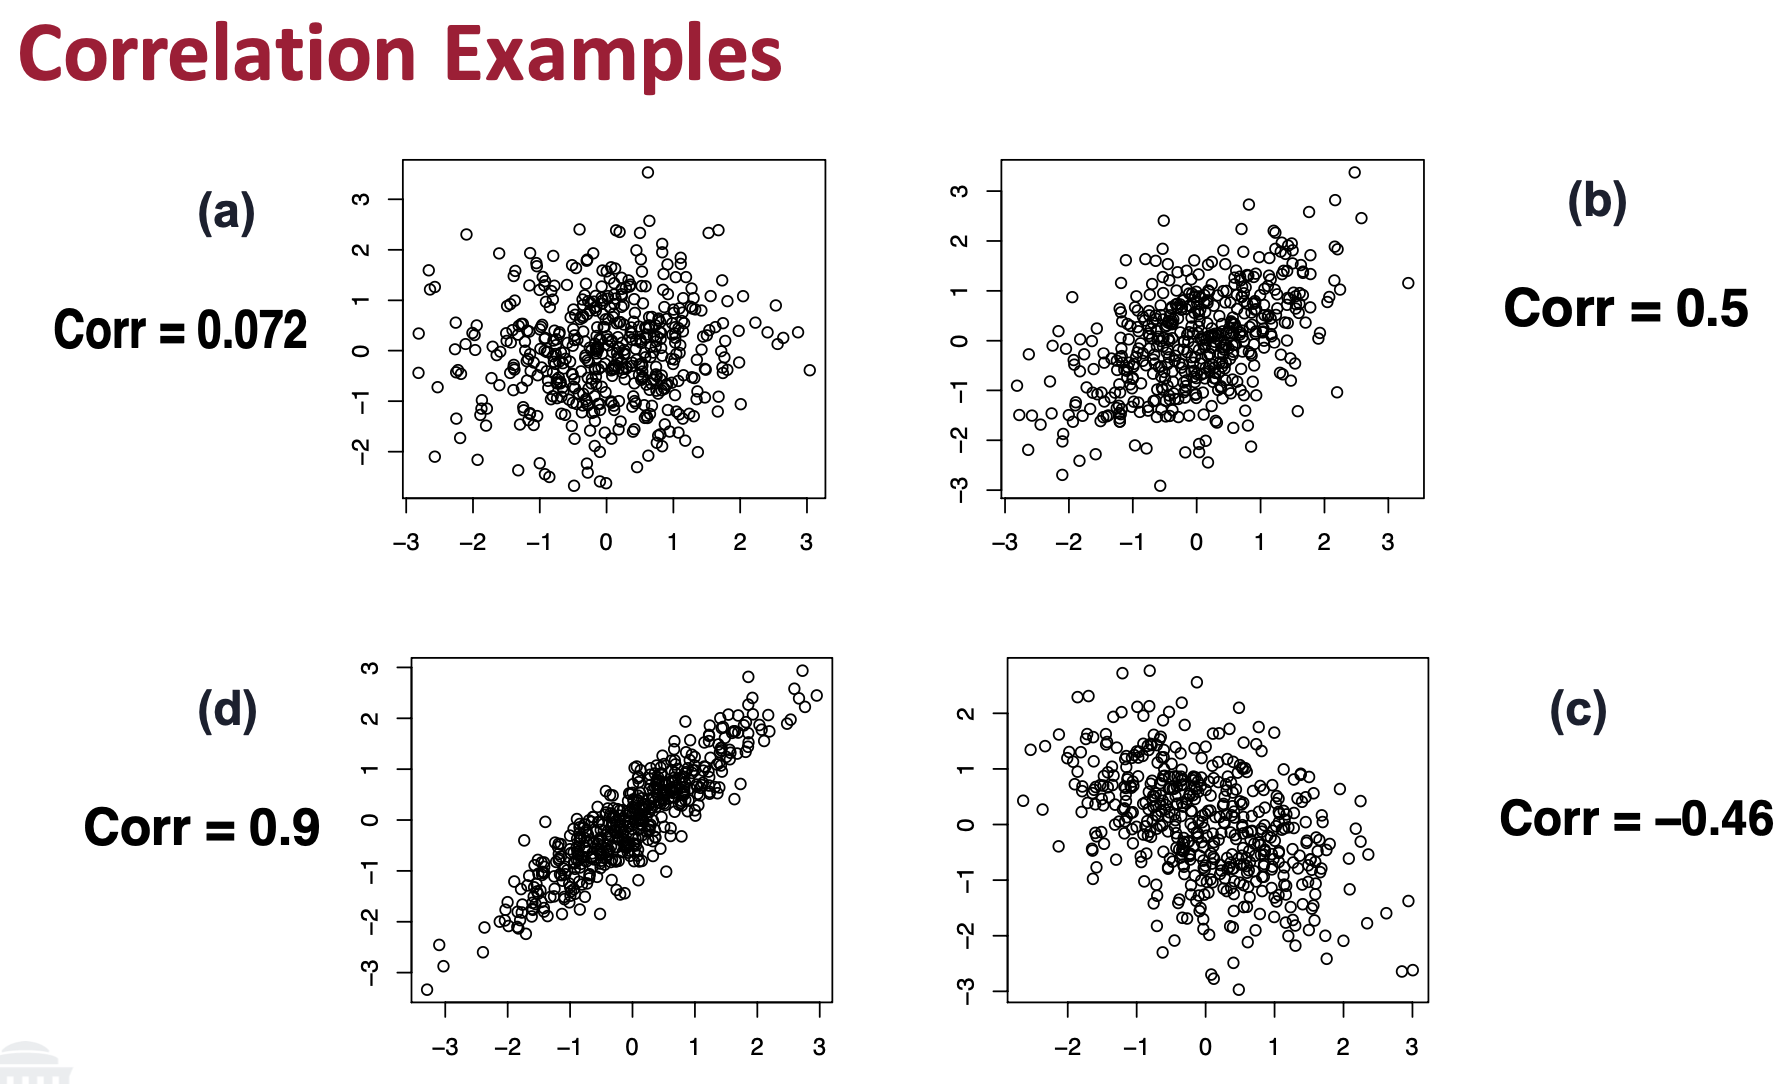
\includegraphics[width=0.25\textwidth]{correlation_examples.png}

\Red{Covariance Between RVs $X$ and $Y$} ``average of the product of the centered variables''. Necessary for assessing variability of sums of RVs (e.g. portfolios).
\begin{displaymath}
    \boxed{
        \begin{aligned}
            \text{Cov}(X, Y) &= \mathbb{E}\left[\left(X - \mathbb{E}[X]\right)\left(Y - \mathbb{E}[Y]\right)\right] \\
            &= \text{Corr}(X, Y) \cdot SD(X) \cdot SD(Y)
        \end{aligned}
    }
\end{displaymath}
\begin{itemize}
    \item $\text{Cov}(X, Y)$ has funny units: product of the $X$ and $Y$ units.
    \item \Hint{$\text{Cov}(X, Y)$ always exists.} If SDs are 0, $\text{Cov}(X, Y) = 0$
    \item $\text{Cov}(X, X) = V(X)$
    \item \Hint{If $SD(X) > 0$ and $SD(Y) > 0$, then $\text{Corr}(X, Y)$ and $\text{Cov}(X, Y)$ have the same sign.}
\end{itemize}

\Green{Expected Value of RVs summed} is regardless of RVs' joint distribution:
\begin{displaymath}
    \boxed{
        \begin{aligned}
            &\mathbb{E}\left[X + Y\right] = \mathbb{E}\left[X\right] + \mathbb{E}\left[Y\right] \\
            &\mathbb{E}\left[X + Y + W\right] = \mathbb{E}\left[X\right] + \mathbb{E}\left[Y\right] + \mathbb{E}\left[W\right] \\
            &\mathbb{E}\left[\sum_{i=1}^{n} X_i\right] = \sum_{i=1}^{n} \mathbb{E}\left[X_i\right] = \mathbb{E}\left[X_i\right] + \dots + \mathbb{E}\left[X_n\right]\\
        \end{aligned}
    }
\end{displaymath}

\Green{Variance of of RVs summed}
\begin{displaymath}
    \boxed{
        \begin{aligned}
            &\text{Var}(X + Y) = \text{Var}(X) + \text{Var}(Y) + 2 \text{Cov}(X, Y) \\
            &\text{Var}(X + Y + W) = \text{Var}(X) + \text{Var}(Y) + \text{Var}(W) \\
            &+ 2 \text{Cov}(X, Y) + 2 \text{Cov}(X, W) + 2 \text{Cov}(Y, W) \\
            &\text{Var}\left(\sum_{i=1}^{n} X_i\right) = \sum_{i=1}^{n} \text{Var}\left(X_i\right) + 2 \sum_{i < j} \text{Cov}(X_i, X_j)
        \end{aligned}
    }
\end{displaymath}
Have to consider the covariance of all possible pairs: $X_i$ and $X_j$.
\Hint{
    \begin{itemize}
        \item If $\text{Corr}(X, Y)$ increases, then $\text{Var}(X + Y)$ increases.
        \item If $V(X) = V(Y)$, then $\text{Var}(X + Y)$ is maximized when $\text{Cov}(X, Y)$ is maximized.
    \end{itemize}
}

\Blue{\underline{Uncorrelated} RVs} if $\text{Corr}(X, Y) = 0$.
Equivalently, they are uncorrelated if $\text{Cov}(X,Y) = 0, SD(X) > 0, SD(Y) > 0$

\Green{Variance of of \underline{Uncorrelated} or \underline{Independent} RVs summed}
\begin{displaymath}
    \boxed{
        \begin{aligned}
            \text{Var}(X + Y) &= \text{Var}(X) + \text{Var}(Y) \\
            \text{Var}\left(\sum_{i=1}^{n} X_i\right) &= \sum_{i=1}^{n} \text{Var}\left(X_i\right)
        \end{aligned}
    }
\end{displaymath}
No change in expected value's formula.

\Blue{\underline{Independent} RVs}
\fbox{$\forall x, y, \mathbb{P}(X = x, Y = y) = \mathbb{P}(X = x)\mathbb{P}(Y = y)$}

\Hint{Independence implies uncorrelatedness}: if two RVs $X$ and $Y$ are independent, then they are uncorrelated.
\fbox{$\text{Independence} \Rightarrow \text{Corr}(X, Y) = 0 = \text{Cov}(X, Y)$}
\Hint{But uncorrelated RVs \underline{can} be dependent!}

\Red{\textit{(iid)} Independent and Identically Distributed RVs}
for a collection of \textit{iid} RVs $\left\{X_1, \dots, X_n\right\}$:
$\forall i \in \{1, \dots, n\}$
\begin{displaymath}
    \boxed{
        \begin{aligned}
            \mathbb{E}[X_i] &= \mu \\
            \text{Var}(X_i) &= \sigma^2 \\
            \text{SD}(X_i) &= \sigma
        \end{aligned}
    }
\end{displaymath}

\Blue{Sum of \textit{iid} RVs} $S_n = X_1 + \dots + X_n$:
\begin{displaymath}
    \boxed{
        \begin{aligned}
            \mathbb{E}[S_n] &= n \cdot \mu \\
            \text{Var}(S_n) &= n \cdot \sigma^2 \\
            \text{SD}(X_i) &= \sqrt{n} \cdot \sigma
        \end{aligned}
    }
\end{displaymath}

\section{Central Limit Theorem (CLT)}
\textbf{If $\left\{X_1, \dots, X_n\right\}$ are \textit{iid} with expected value $\mathbb{E}[X_i] = \mu$ and variance $\text{Var}(X_i) = \sigma^2 < \infty$},
then as $n \rightarrow \infty$:
\begin{itemize}
    \item $S_n \sim \mathcal{N}(n \cdot \mu, \sqrt{n} \cdot \sigma)$
    \item $\text{Mean}_n \sim \mathcal{N}(\mu, \frac{\sigma}{\sqrt{n}})$
\end{itemize}
\Hint{If $n$ is large enough (heuristic: \underline{$n > 30$}), we can calculate probabilities for the sum and mean of RVs by using the normal distribution.}

\Green{Emperical Rules under CLT}
\begin{itemize}
    \item 50\% of the time,\begin{itemize}
        \item $S_n$ will fall within $n\mu \pm \frac{2}{3}\sqrt{n} \sigma$
        \item $M_n$ will fall within $\mu \pm \frac{2}{3}\frac{\sigma}{\sqrt{n}}$
    \end{itemize}
    \item 68\% of the time,\begin{itemize}
        \item $S_n$ will fall within $n\mu \pm \sqrt{n} \sigma$
        \item $M_n$ will fall within $\mu \pm \frac{\sigma}{\sqrt{n}}$
    \end{itemize}
    \item 95\% of the time,\begin{itemize}
        \item $S_n$ will fall within $n\mu \pm 2\sqrt{n} \sigma$
        \item $M_n$ will fall within $\mu \pm 2\frac{\sigma}{\sqrt{n}}$
    \end{itemize}
    \item 99.7\% of the time,\begin{itemize}
        \item $S_n$ will fall within $n\mu \pm 3\sqrt{n} \sigma$
        \item $M_n$ will fall within $\mu \pm 3\frac{\sigma}{\sqrt{n}}$
    \end{itemize}
\end{itemize}

\section{Sampling and Confidence Intervals}

\Red{Confidence Interval} contains an unknown (population) quantity at some specified sampling frequency.
\begin{itemize}
    \item Confidence intervals \Hint{do not} depend on population size, but only on sample size.
    \item For a given sample size, can be very precise with low confidence or very imprecise with high confidence.
    \item 2x the precision requires 4x sample size; 3x the precision requires 9x sample size.
\end{itemize}

Wording matters...
\begin{itemize}
    \item OK: ``I am 95\% confident the interval [a,b] contains the true population proportion''
    \item OK: ``There is a 95\% probability the interval [a,b] contains the true population proportion''
    \item Not OK: ``There is a 95\% probability the true population proportion lies in the interval [a,b]''
\end{itemize}

\Green{Confidence Level ($L$) to $c$}
\fbox{$c = \texttt{qnorm}(p = \frac{(1 + L)}{2}, \mu = 0, \sigma = 1)$}
(find the value $c$ such that the area under $\mathcal{N}(\mu, \sigma)$ is $p$)
\begin{center}
    \begin{tabular}{ c|c|c } 
        confidence level & $L$ & $c$ \\ 
        \hline
        90\% & 0.9 & 1.65 \\ 
        95\% & 0.95 & 1.96 \\ 
        99\% & 0.99 & 2.58 \\ 
    \end{tabular}
\end{center}
    
\Blue{For a population \underline{mean}} Given sample size $n$, sample average $\bar{x}$, and sample standard deviation
$s$, we are X\% confident the true population mean lies in the interval:
\fbox{$\bar{x} \pm \left(c \frac{s}{\sqrt{n}}\right)$} ``MOE'': $\left(c \frac{s}{\sqrt{n}}\right)$

\Blue{For a population \underline{proportion}} Given sample size $n$, sample proportion $\bar{p}$, and
\Hint{standard deviation in the population to be $0.5$}, we are X\% confident the true population mean lies in the interval:
\fbox{$\bar{p} \pm \left(c \frac{0.5}{\sqrt{n}}\right)$} ``MOE'': $\left(c \frac{0.5}{\sqrt{n}}\right)$

\Hint{Important assumptions:}
\begin{itemize}
    \item Sample is random
    \item Sample is large enough ($n > 30$) for CLT
    \item The worst possible standard deviation in the population to be $0.5$
\end{itemize}

\Red{Sampling Distribution} is well approximated by
$\mathcal{N}(\mu = \text{true population parameter}, \sigma = \frac{\text{population SD}}{\sqrt{n}})$, based on CLT.
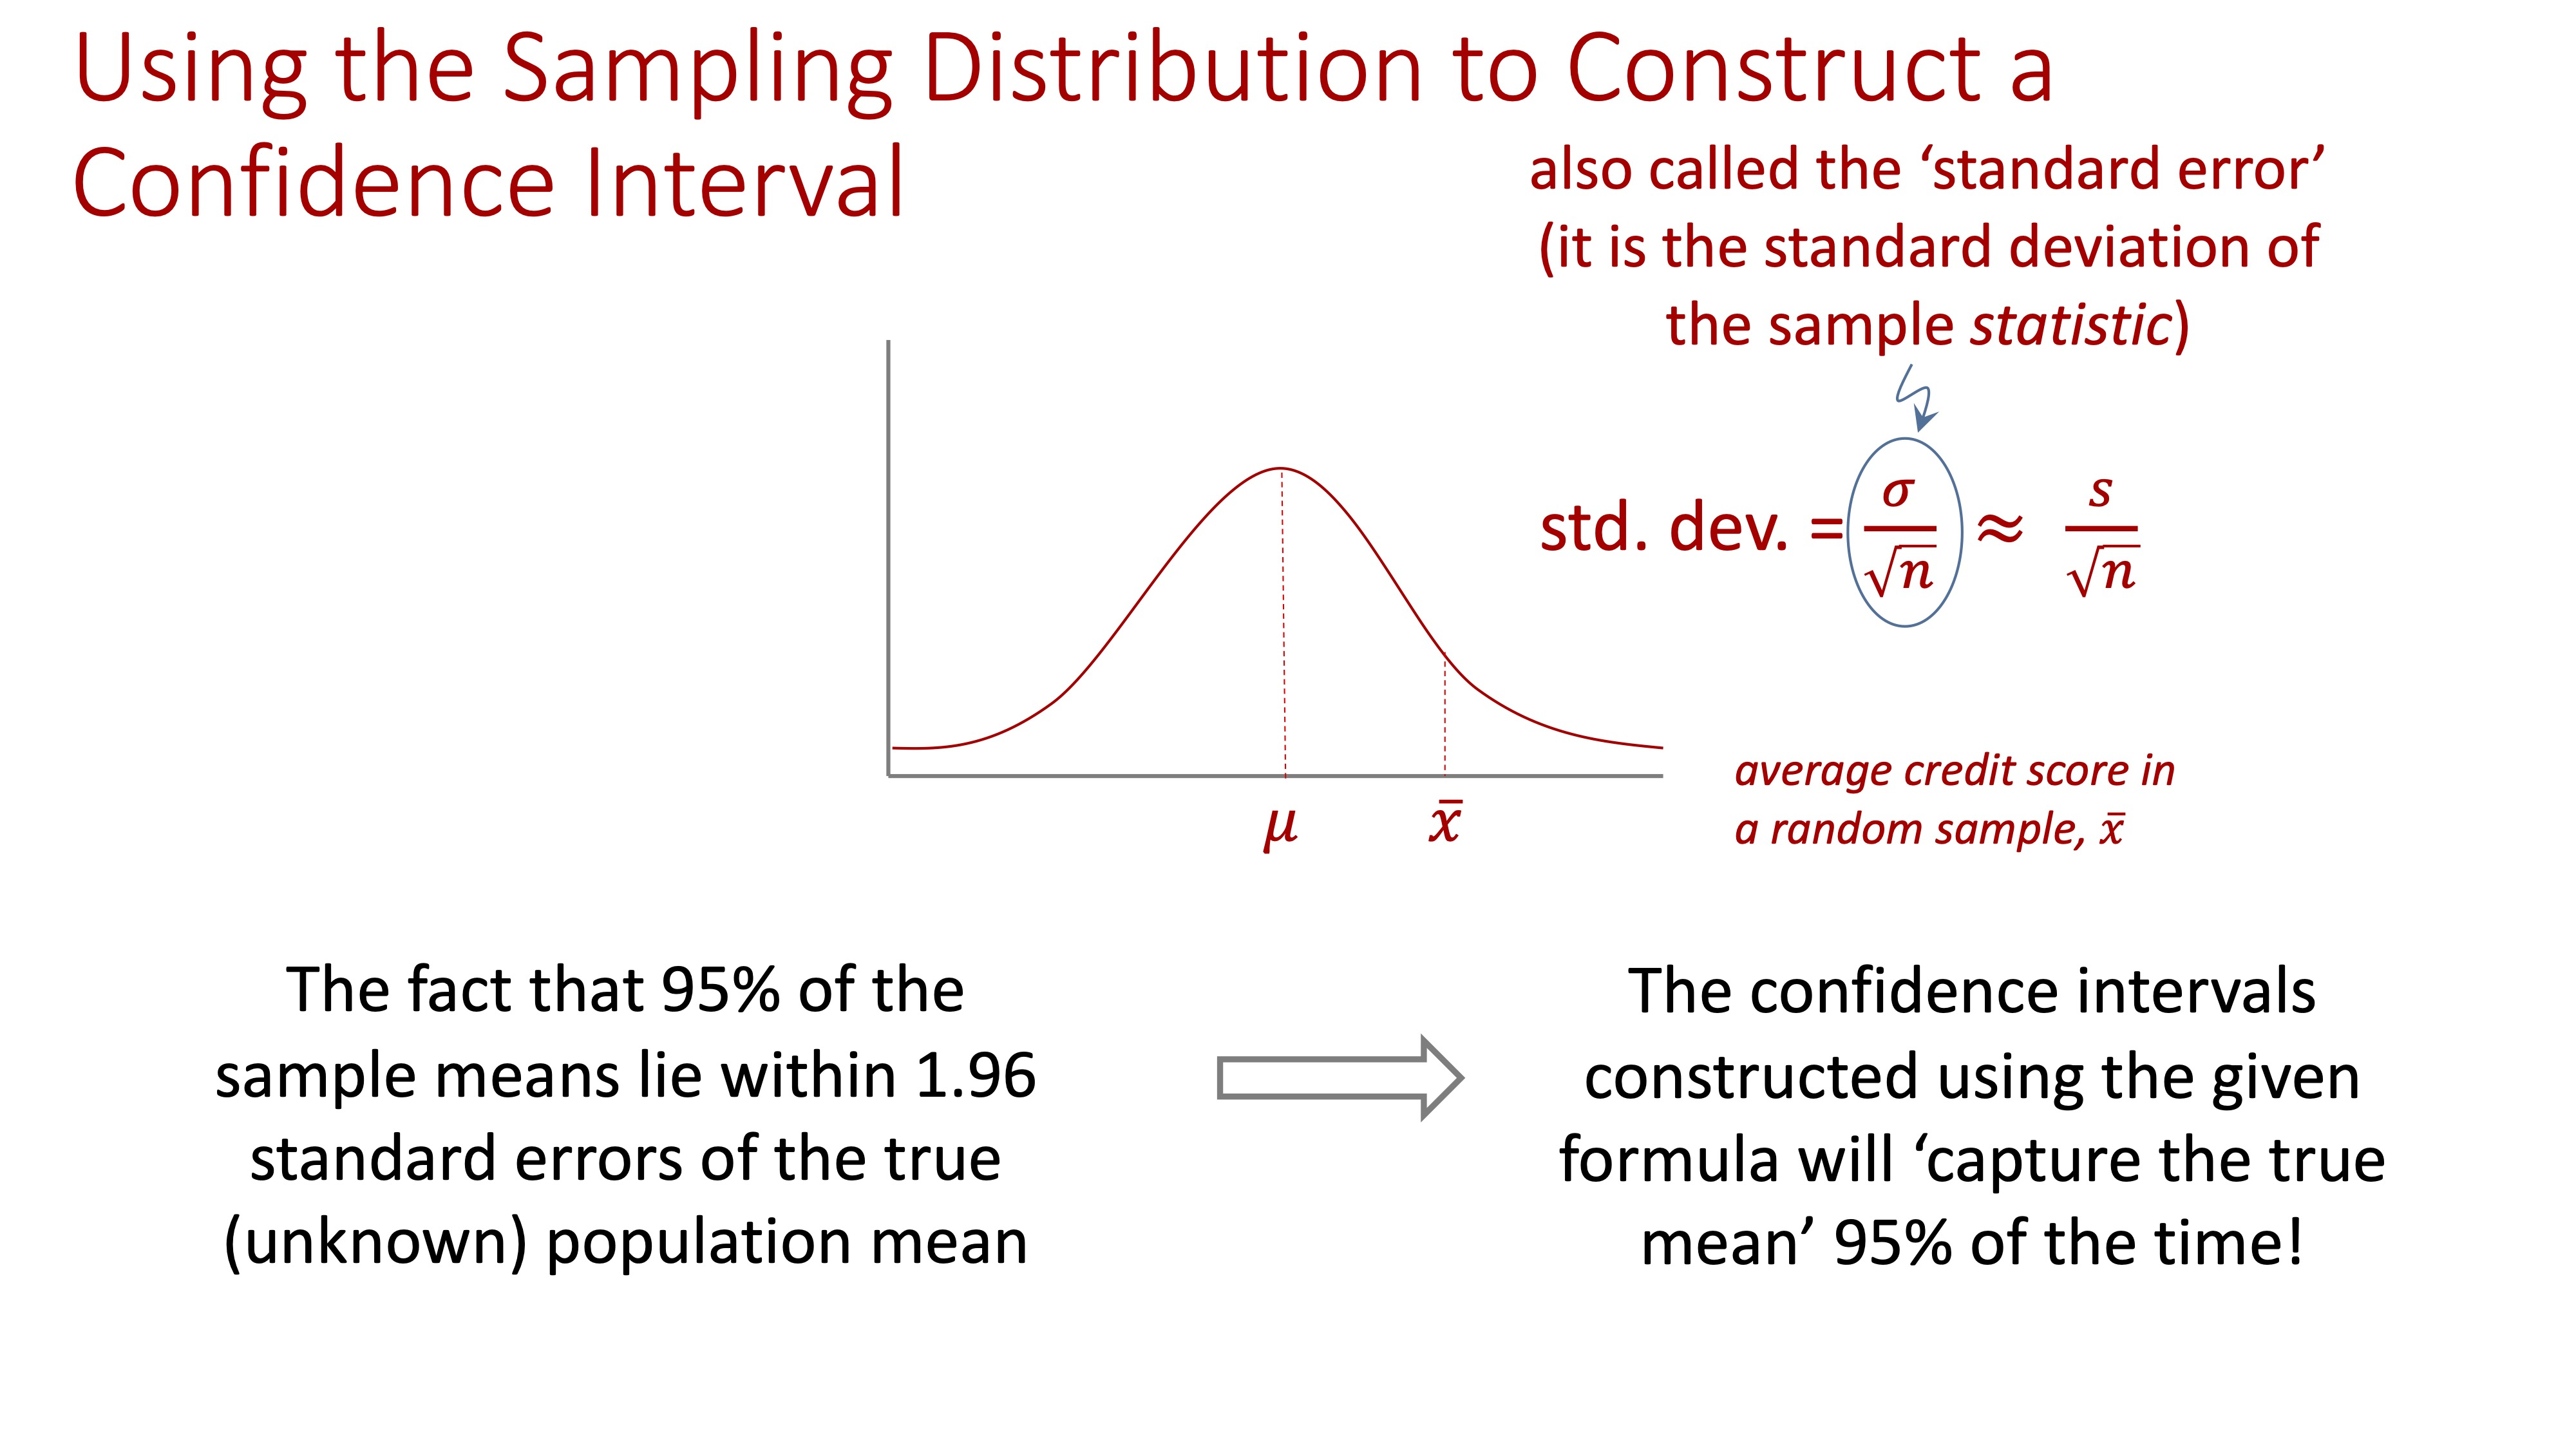
\includegraphics[width=0.253\textwidth]{standard_error.jpg}
\Hint{Take away:} assuming a conservative confidence interval based on $0.5$ is \underline{not} the only way!
Can estimate standard error using the surveyed proportion too.
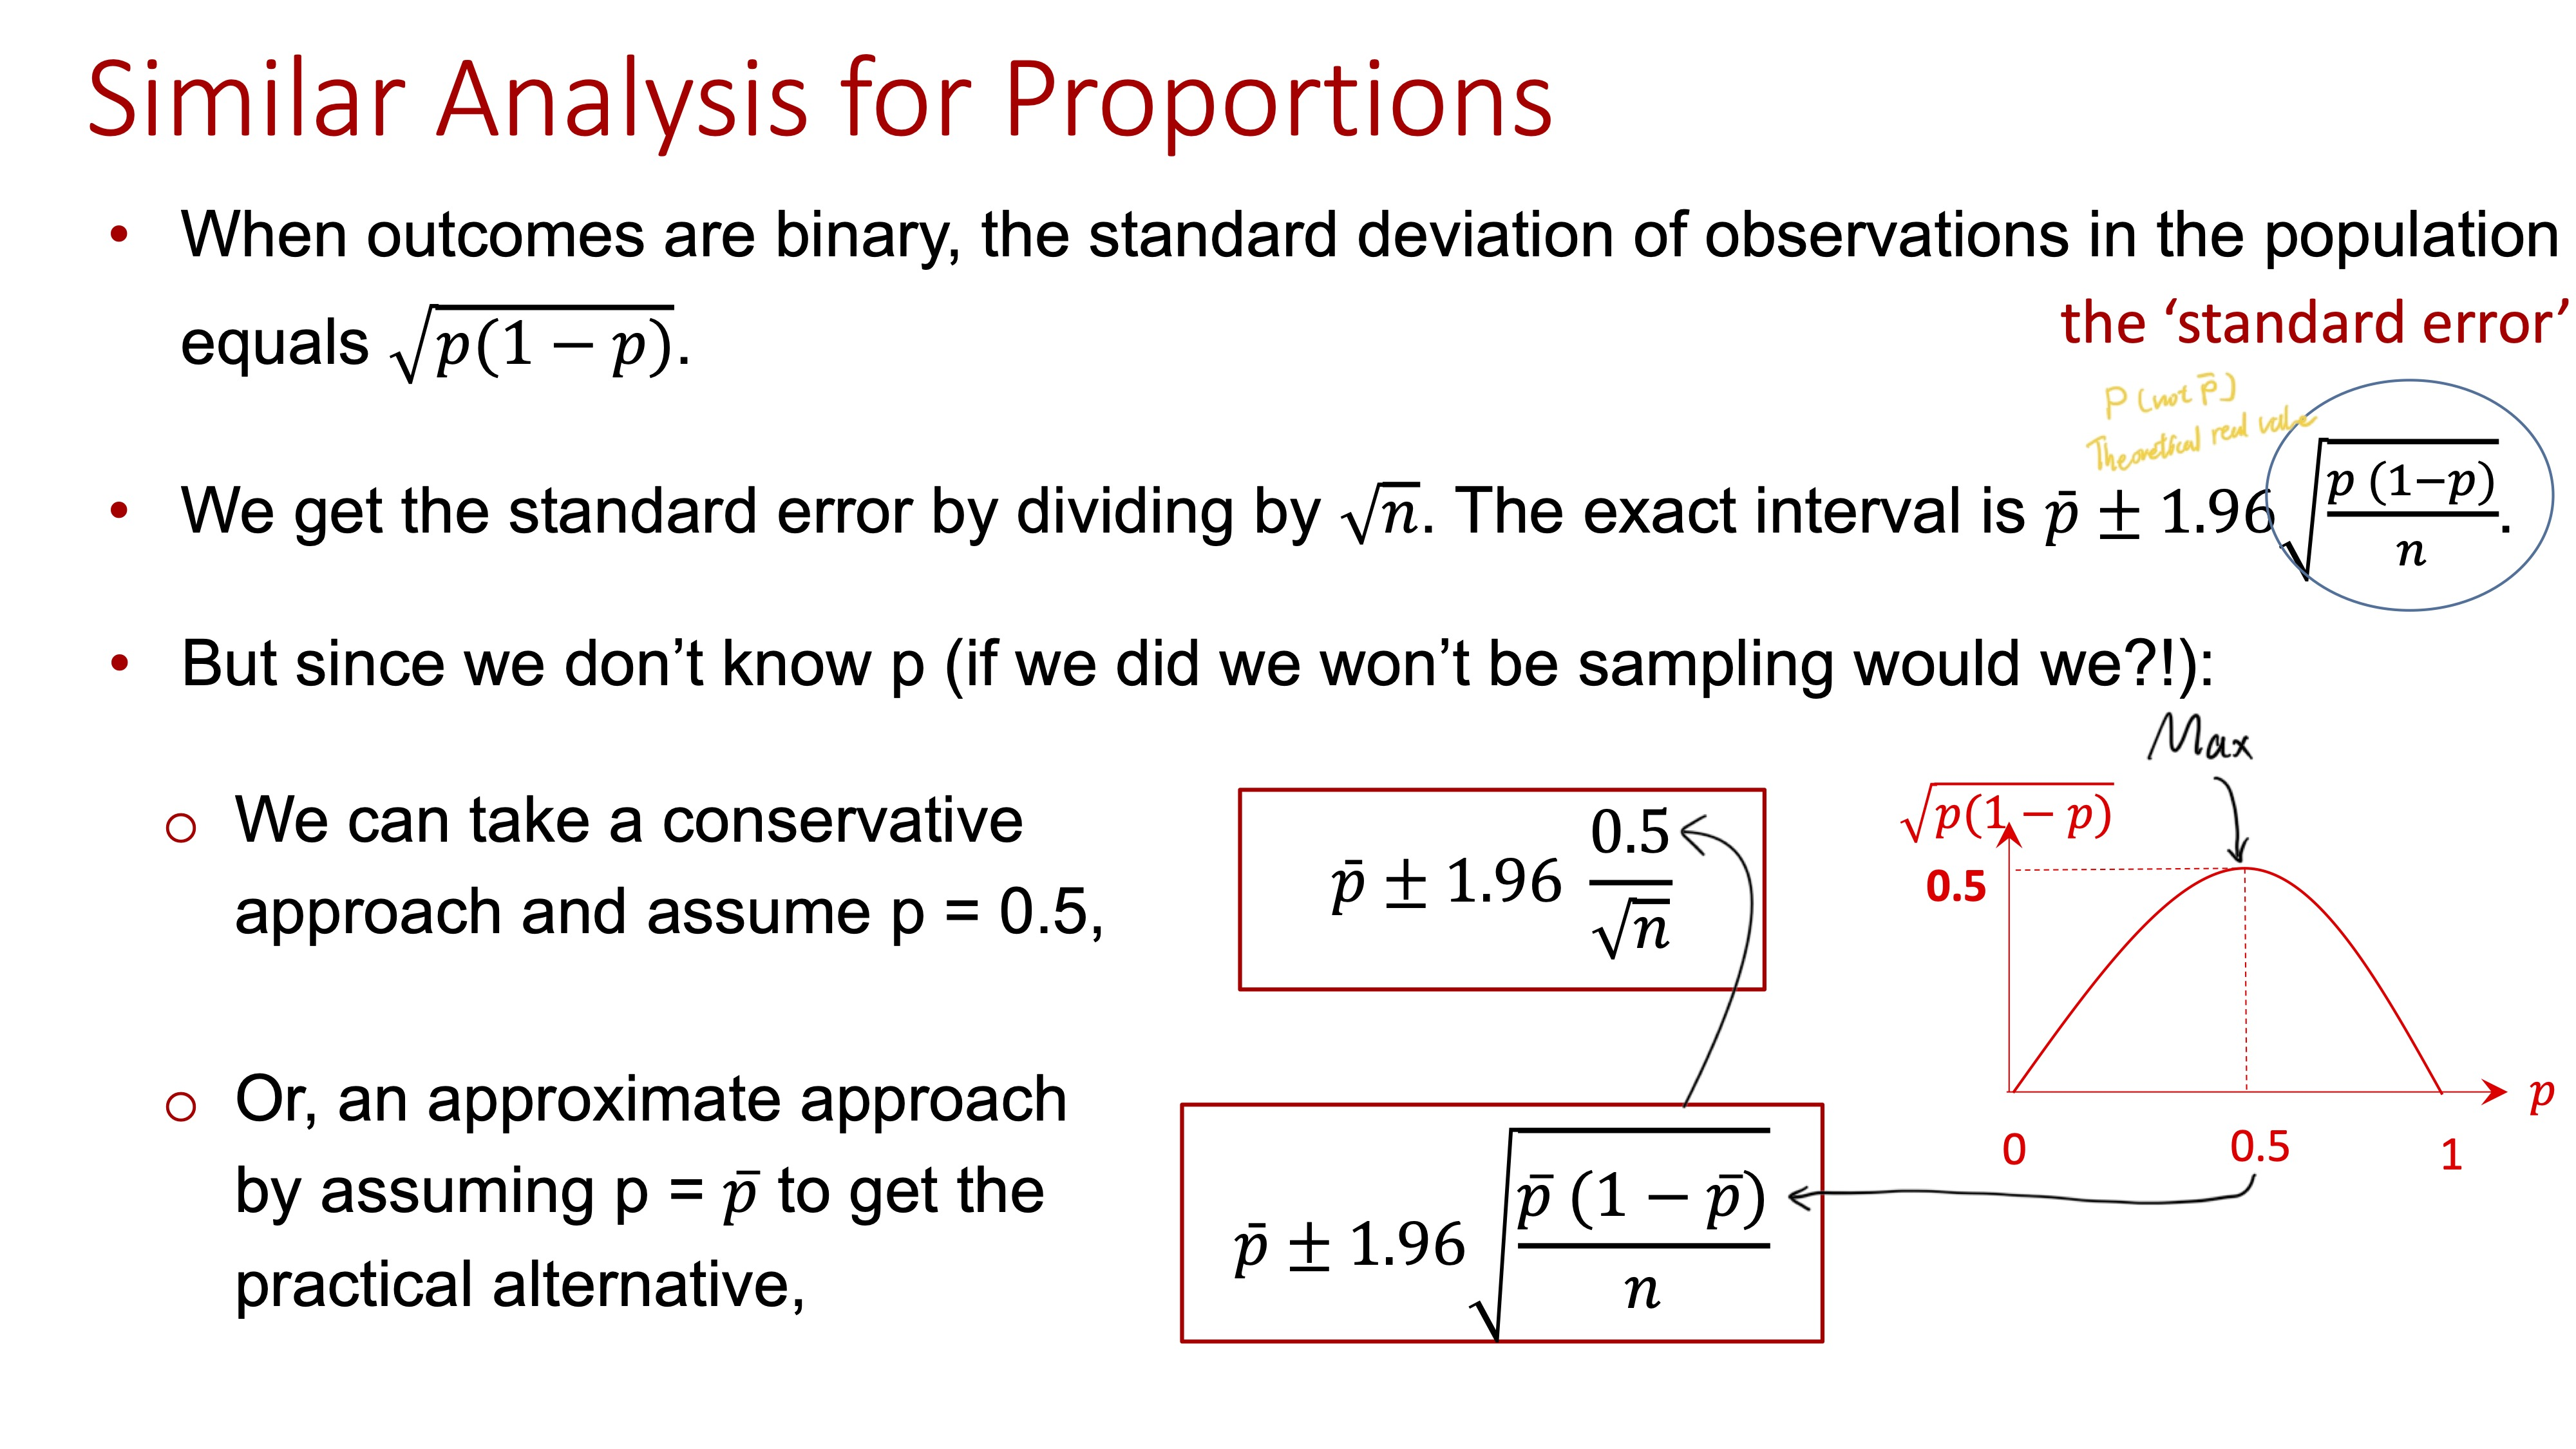
\includegraphics[width=0.253\textwidth]{proportions.jpg}

\Blue{Sampling Errors} the sample-to-sample variations due to pure chance. MOE and confidence intervals quantify this
uncertainty well.

\Blue{Non-Sampling Errors} (some examples)
\begin{itemize}
    \item Selection Bias: happens when each member of the population does not have the same chance of being selected.
    \item Response/Non-response Bias: happens when some fraction of the individuals surveyed don’t respond for reasons related to what’s being asked in the survey
\end{itemize}

\section{R Distribution Functions}
    
\begin{itemize}
    \item \texttt{p} (``probability''): cumulative distribution function (“what is the probability above or below a cutoff?”)
    \item \texttt{q} (``quantile''): inverse CDF (“what value do we find at, say, 80\% of the way to the maximal value?”)
    \item \texttt{d} (``density''): density function (gives us the “height” or y-value of distribution for a particular z-score - mainly useful in plotting)
\end{itemize}

\lstset{breaklines=true}
\begin{lstlisting}[language=R]
# Exactly k successes in n trials given success probability p
dbinom(k, size=n, p=p)
# k or more successes in n trials given success probability p
sum(dbinom(k:n, size=n, p=p))

# Probability of this value or less
pnorm(value, mean, sd)
# Probability of this value or greater
pnorm(value, mean, sd, lower.tail=FALSE)
# Highest value associated with a given percentile
qnorm(percentile, mean, sd)

\end{lstlisting}

\end{multicols}
\end{document}